\chapter{Evaluation of radiation}\label{evaluation}
In current version of the code following types of radiation are implemented: synchrotron radiation, inverse Compton scattering, gamma-ray emission due to pion decay in free-free proton interaction and also bremsstrahlung.

Abstract class RadiationEvaluator and it's inherited classes are used for evaluation of radiation. There are derved classes for every specific type of radiation and also class RadiationSumEvaluator which allows to sum several different types of radiation. Public methods of this two classes are listed in Table \ref{radiationEvaluator}. 

General approach to evaluation of radiation is following: create radiation source, using one of the classes, described in Section \ref{sourcesSection}, or user-defined, then create object of radiation evaluator, which types are described below, and then call method evaluateFluxFromSource(const double\& photonFinalEnergy, RadiationSource* source) of this object, which evaluates energy density of the energy flux from source in units $\rm cm^{-2} s^{-1}$.

\begin{figure}[h]
	\centering
	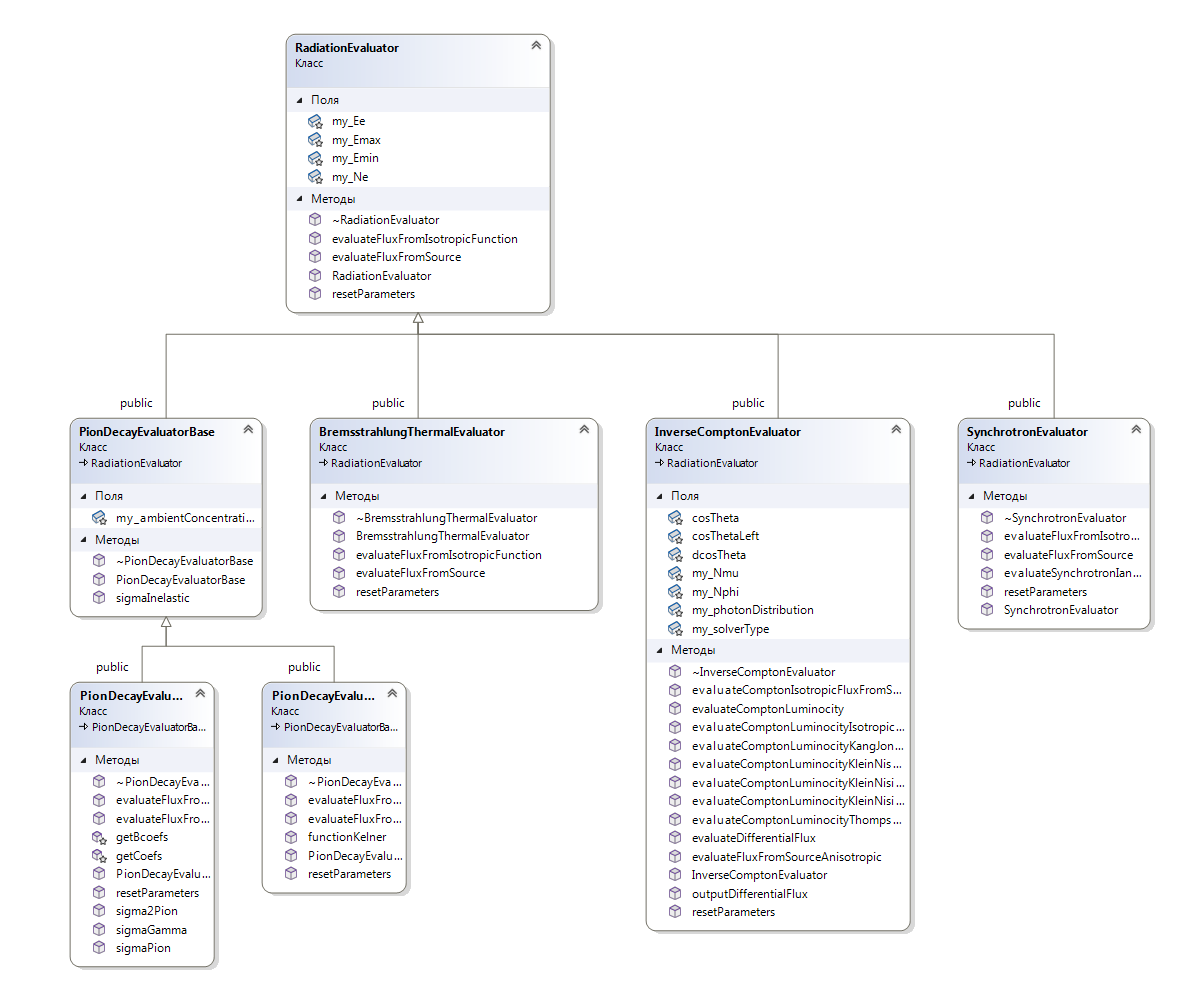
\includegraphics[width=10.5 cm]{./fig/radiationEvaluator.png} 
	\caption{class hierarchy of radiation evaluators}
	\label{radiationEvaluators}
\end{figure}

Classes for every specific type of electromagnetic radiation are described below in this chapter. Class hierarchy of radiation evaluators is shown in Figure \ref{radiationEvaluators}. Equations used for evaluation are discussed in Chapter \ref{Formulae}.

\begin{small}
	\topcaption{Public methods of RadiationEvaluator class}
	\label{radiationEvaluator}
	\begin{xtabular}{|p{0.51\textwidth}|p{0.49\textwidth}|} 
		\hline
		\textbf{RadiationEvaluator} & astract class for evaluation of radiation \\
		\hline
		virtual evaluateFluxFromSource(const double\& photonFinalEnergy, RadiationSource* source) & virtual method, returns energy density of radiation energy flux in units $\text{cm}^{-2} \text{s}^{-1}$ \\
		\hline
		virtual double evaluateFluxFromSourceAtPoint(const double\& photonFinalEnergy, RadiationSource* source, int rhoi, int phi) & virtual method, returns energy density of radiatio energy flux from given grid cell on tangent plane\\
		\hline
		double evaluateTotalFluxInEnergyRange(const double\& Ephmin, const double\& Ephmax, int Nph, RadiationSource* source) & returns integrated energy flux in the given energy range, evaluted by Nph points distributied logarithmically, in units $\text{erg} \text{cm}^{-2} \text{s}^{-1}$\\
		\hline
		virtual resetParameters( const double* parameters, const double* normalizationUnits) & virtual method, reseting parameters of the radiation evaluator. Lists of parameters are different for different types of evaluators. Method takes for input array of parameters in normalized units, and array of normalization conctants. This method for example is used for fitting modelled radiation to the observational data and optimization.\\
		\hline
		writeFluxFromSourceToFile(const char* fileName, RadiationSource* source, const double\& Ephmin, const double\& Ephmax, const int Nph) & evaluates and writes into the file energy density of radiation energy flux in given energy range with Nph points distributed logarithmically. Writes two columns of data in units $\text{erg}$  and $\text{cm}^{-2} \text{s}^{-1}$\\
		\hline
		writeImageFromSourceToFile(const char* fileName, RadiationSource* source, const double\& Ephmin, const double\& Ephmax, const int Nph) & evaluates and writes to file image - energy flux from every cell of the tangent plane in units $\text{erg} \text{cm}^{-2} \text{s}^{-1}$ integrated in given energy range with Nph points distributed logarithmically\\
		\hline
		writeImageFromSourceAtEToFile(const double\& photonFinalEnergy, const char* fileName, RadiationSource* source) & evaluates and writes to file image - energy density of radiation energy flux from every cell of the tangent plane in units $\text{cm}^{-2} \text{s}^{-1}$\\
		\hline
		\textbf{RadiationSumEvaluator} & class for sum of several types of radiation\\
		\hline
		RadiationSumEvaluator(int Ne, const double\& Emin, const double\& Emax, RadiationEvaluator* evaluator1, RadiationEvaluator* evaluator2) & constructor, creates evaluator which sums results of two given evaluators, and takes into accaunt emmiting particles in given energy range\\
		\hline
		RadiationSumEvaluator(int Ne, const double\& Emin, const double\& Emax, int Nev, RadiationEvaluator** evaluators) & constructor, creates evaluator which sums results of given array of evaluators, and takes into accaunt emmiting particles in given energy range\\
		\hline
	\end{xtabular}
\end{small}

\section{Synchrotron radiation}\label{synchrotronSection}
Class SynchrotronEvaluator is implemented for evaluation of synchrotron radiation. It uses standard approximation of continious spectrum, described in \cite{Ginzburg1975, Ghisellini} and in section \ref{synchrotronFormulaSection},  - it is valid for frequencies of emitted photons much higher than gyrofrequency of emitting particles. Also it is possible to take into account synchrotron self-absorption. Cylindrical geomtry, shown in Figure \ref{sphericalLayer} allows to integrate flux through the line of sight and take into account absorption inside the source. To create SynchrotronEvaluator object user should provide energy range of particles to be taken into account, numbers of integration points in it, and also two boolean parameters - for accounting self absorption and doppler shifting due to source matter velocity. Public methods of Synchrotron evaluator are listed in Table  \ref{SynchrotronEvaluator}. Example of evaliation of synchrotron radiation is shown in section \ref{quickStart}.
\begin{table}[h]
	\begin{center}
	\begin{small}
	\caption{Public methods of SynchrotronEvaluator}
	\label{SynchrotronEvaluator}
	\begin{tabularx}{\textwidth}{|X|X|} 
		\hline
		\textbf{SynchrotronEvaluator} & class for evaluation synchrotron radiation\\
		\hline
		SynchrotronEvaluator( int Ne, double Emin, double Emax, bool selfAbsorption = true, bool doppler = false) & constructor, creates evaluator with given energy range of particles taken into account and parameters corresponding to self-absorption and doppler effect\\
		\hline
		evaluateSynchrotronIandA(const double\& photonFinalFrequency, const double\& photonFinalTheta, const double\& photonFinalPhi, const double\& B, const double\& sinhi, const double\& concentration, MassiveParticleIsotropicDistribution* electronDistribution, double\& I, double\& A) & evaluates emissivity per unit volume and absorption coefficient for photon of given energy and direction in given magnetic field and number density and distribution of emitting particles\\
		\hline
	\end{tabularx}
\end{small}
\end{center}
\end{table}
\section{Inverse Compton scattering}
Class InverseComptonEvaluator is implemented for evaluation of radiation produced in inverce compton scattering. Also it has one derived class InverseComptonEvaluatorWithSource. The difference between them is that in the first one distribution of seed photons is constant inside the source, and in the second one photons number density is change proportionaly inverse square of the distance to the source of seed photons.

There are four different algorithmes of evaluation IC radiation that can be used by InverseComptonEvaluator. They are listed by enum-type ComptonSolverType, having following values:

\begin{itemize}
	\item ISOTROPIC\_THOMSON - simple model of scattering in thomson regime with power-law distribution of electrons and thermal distribution of seed photons, as described in \cite{Ginzburg1975} ch 17, p. 466.
	\item ANISOTROPIC\_KLEIN\_NISHINA - model computing radiation directly by integrating Klein-Nishina cros-section as described in \cite{KleinNishina, Dubus} and in section \ref{comptonFormulaSection}. With this model is possible to evaluate radiation produced by anisotropic distributions of initial particles
	\item ISOTROPIC\_KLEIN\_NISHINA - model similar to the previous, it uses integration of Klein-Nishina cross-section, but isotropy of distributions of initial particles is assumed, and it allows to reduce number of integrations through the azimuthal angle
	\item ISOTROPIC\_JONES - model, using analytical integration through the all angular variables, in case of isotropic distributions of initial particles. It is described in \cite{JonesCompton, BykovUvarov2000} and in section??
\end{itemize}

To create object of InverseComptobEvaluator type user needs to provide energy range of particles taken into account and nimber of points to integrate through it, number of points through the polar and azimutal angle, distribution function of seed photons and algorithm of computation the radiation. Public methods of InverseComptonEvaluator and InverseComptonEvaluatorWithSource are listed in Table \ref{InverseComptonEvaluator}.
\begin{small}
	\topcaption{Public methods of inverse compton scattering evaluators}
	\label{InverseComptonEvaluator}
	\begin{xtabular}{|p{0.5\textwidth}|p{0.5\textwidth}|} 
		\hline
		\textbf{InverseComptonEvaluator} & class for evaluation radiation from inverse compton scattering\\
		\hline
		InverseComptonEvaluator( int Ne, int Nmu, int Nphi, double Emin, double Emax, PhotonDistribution* photonDistribution, ComptonSolverType solverType) & constructor, creates evaluator with given energy range of particles taken into account, numbers of integration points throught the energy and angular variables, distribution function of seed photons and method of computation the radiation\\
		\hline
		evaluateFluxFromSourceAnisotropic( const double\& photonFinalEnergy, const double\& photonFinalTheta, const double\& photonFinalPhi, PhotonDistribution* photonDistribution, RadiationSource* source) & returns energy density of radiation energy flux created by given seed photons distribution and source containing scattering particles in given direction\\
		\hline
		evaluateTotalFluxInEnergyRangeAnisotropic( const double\& Ephmin, const double\& Ephmax, const double\& photonFinalTheta, const double\& photonFinalPhi, int Nph, PhotonDistribution* photonDistribution, RadiationSource* source, ComptonSolverType solverType) & returns total energy flux of radiation created by given seed photons distribution and source containing scattering particles in given direction integrated in given energy range through Nph point distributed logarithmically.\\
		\hline
		\textbf{InverseComptonEvaluatorWithSource} & class for evaluation radiation from inverce comton scattering takin into account dependency of photons number density on distance to the source of photons\\
		\hline
		InverseComptonEvaluatorWithSource(int Ne, int Nmu, int Nphi, double Emin, double Emax, double Ephmin, double Ephmax, PhotonDistribution* photonDistribution, ComptonSolverType solverType, const double\& sourceR, const double\& sourceZ, const double\& sourcePhi) & constructor, creates evaluator with given energy range of particles taken into account, numbers of integration points throught the energy and angular variables, distribution function of seed photons with number density corresponding to the origin of coordinates, method of computation the radiation and coordinates of the source of seed photons\\
		\hline
	\end{xtabular}
\end{small}

Example of the evaluation of radiation produced by Inverse Compton scattering is shown in the function  evaluateComtonWithPowerLawDistribution() in the file examples.cpp. In this function X-ray radiation from Fast Blue Optical Transient CSS161010 is evaluated. Electrons distribution is assumed power-law as in paper \cite{Coppejans2020} and seed photons are taken from mean galactic photon field \cite{Mathis1983}.

At first let define main parameters of the source - it's size, distance to observer, electrons number density and magnetic field. Magnetic field doesn't matter for inverse compton scattering, so assume it equal to zero. Also we define numbers of grid points for integration through the energy and angular variables

\begin{lstlisting}[language=c++]
	double electronConcentration = 150;
	double sinTheta = 1.0;
	double rmax = 1.3E17;
	double B = 0.0;
	double distance = 150*1E6*parsec;
	
	double Emin = me_c2;
	double Emax = 1000 * me_c2;
	int Ne = 200;
	int Nmu = 20;
	int Nphi = 4;
\end{lstlisting}

Then we create distribution of seed photons, using static method of class MultiPlankDistribution getGalacticField wich returns mean galactic photon distribution. And also we create electron power-law distribution with spectral index 3.5

\begin{lstlisting}[language=c++]
	PhotonIsotropicDistribution* photonDistribution = 
	    PhotonMultiPlankDistribution::getGalacticField();
	MassiveParticlePowerLawDistribution* electrons = new 
	    MassiveParticlePowerLawDistribution(massElectron, 3.5,
	    Emin, electronConcentration);
\end{lstlisting}

Then we create radiation source as homogenous disk and radiation evaluator for inverse Compton scattering. Let use the most universal method of comutation inverse compton radiation - ANISOTROPIC\_KLEIN\_NISHINA

\begin{lstlisting}[language=c++]
	RadiationSource* source = new SimpleFlatSource(
	  electrons, B, sinTheta, rmax, rmax, distance);
	
	InverseComptonEvaluator* comptonEvaluator = new 
	    InverseComptonEvaluator(Ne, Nmu, Nphi, Emin, Emax, 
	    photonDistribution, ComptonSolverType::ANISOTROPIC_KLEIN_NISHINA);
\end{lstlisting}

If user don't want to use standard method to writing radiation in to the file, in case of one need result in some other units - electron-volts for energy and write energy density flux in units 
$E F(E)$ - $\text{erg}~\text{cm}^{-2}\text{s}^{-1}$, user should write result to file manually. Let create grid for energy of radiated photons
\begin{lstlisting}[language=c++]
	int Nnu = 200;
	double* E = new double[Nnu];
	double* F = new double[Nnu];
	double Ephmin = 0.01 * kBoltzman * 2.725;
	double Ephmax = 2 * Emax;
	double factor = pow(Ephmax / Ephmin, 1.0 / (Nnu - 1));
	E[0] = Ephmin;
	F[0] = 0;
	for (int i = 1; i < Nnu; ++i) {
		E[i] = E[i - 1] * factor;
		F[i] = 0;
	}
\end{lstlisting}
and then compute energy density fluxes for this energies
\begin{lstlisting}[language=c++]
	for (int i = 0; i < Nnu; ++i) {
		F[i] = comptonEvaluator->evaluateFluxFromSource(
		    E[i], source);
	}
\end{lstlisting}
and wrtie them to file transforming to the prefered units
\begin{lstlisting}[language=c++]
	FILE* output_ev_EFE = fopen("output.dat", "w");
	
	for (int i = 0; i < Nnu; ++i) {
		fprintf(output_ev_EFE, "%g %g\n",
		    E[i] / (1.6E-12), E[i] * F[i]);
	}

	fclose(output_ev_EFE);
\end{lstlisting}
Spectrum of radiation, obtained with this code is shown in Figure \ref{compton}
\begin{figure}[h]
	\centering
	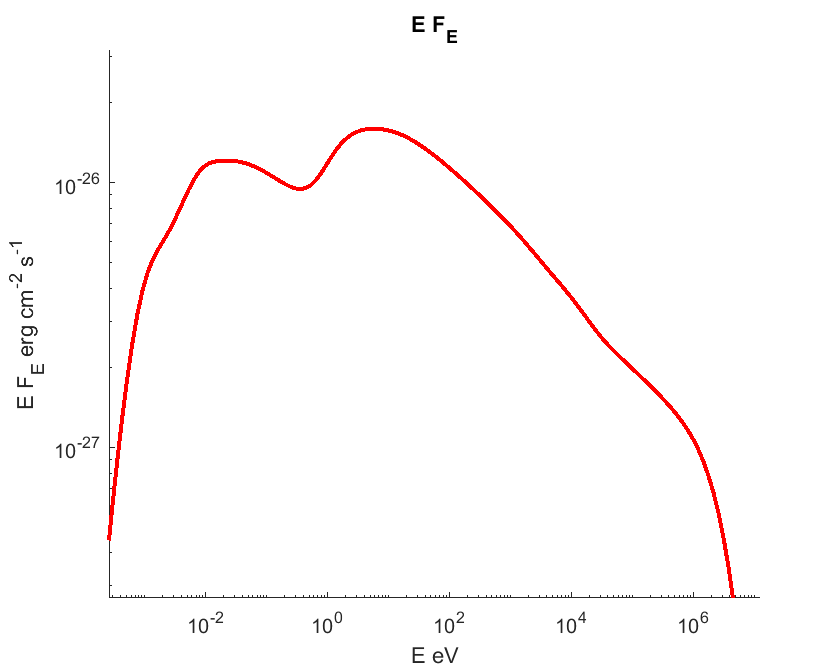
\includegraphics[width=12.5 cm]{./fig/compton.png} 
	\caption{Energy density flux of inverse compton radiation}
	\label{compton}
\end{figure}

\section{Распад пионов}

Для расчета излучения, получающегося в результате распада пионов, родившихся в результате свободно-свободного взаимодействия протонов использеутся абастрактный класс PionDecayEvaluatorBase и двае его наследника: PionDecayEvaluatorKelner, в котором сечение излучения гамма-фотона считается долей от полного сечения неупругого взаимодействия протонов, как описано в статье \cite{Kelner}, и PionDecayEvaluator, в котором используется более точное описание сечения рождения пионов на низких энергиях по методу, описанному в \cite{Kafexhiu}. В текущей версии предполагается, что характерное время потерь энергии протонов при неупругом взаимодействии намного больше времени их удержания в источнике, система является прозрачной для протонов, и каждый из них взаимодействует не более одного раза. В противном случае используемая модель излучения не применима.

При создании объекта класса PionDecayEvaluator необходимо указать рассматриваемый диапазон энергий частиц и количество точек в нем, а так же концентрацию фоновых протонов, так как предполагается рассеяние высокоэнергичных фотонов на покоящихся, а не взаимодействие высокоэнергичных между собой. Публичные методы класса PionDecayEvaluatorBase и его наследников приведены в Таблице \ref{pionDecay}

		\begin{small}
			\topcaption{Публичные методы классa PionDecayEvaluatorBase и его наследников }
			\label{pionDecay}
			\begin{xtabular}{|p{0.5\textwidth}|p{0.5\textwidth}|}  
				\hline
				\textbf{PionDecayEvaluatorBase} & абстрактный класс для вычисления гамма излучения от распада пионов\\
				\hline
				sigmaInelastic(const double\& energy) & возвращает полное сечение неупругого взаимодействия протонов в лабораторной системе, принимает кинетическую энергию движущегося протона\\
				\hline
				\textbf{PionDecayEvaluatorKelner} & класс для вычисления гамма излучения от распада пионов по методу из статьи \cite{Kelner}\\
				\hline
				PionDecayEvaluatorKelner(int Ne, double Emin, double Emax, const double\& ambientConcentration) & конструктор, создает экземпляр с заданным рассматриваемым диапазоном энергии и концентрацией фоновых протонов\\
				\hline
				\textbf{PionDecayEvaluator} & класс для вычисления гамма излучения от распада пионов по методу из статьи \cite{Kafexhiu}\\
				\hline
				PionDecayEvaluator(int Ne, double Emin, double Emax, const double\& ambientConcentration) & конструктор, создает экземпляр с заданным рассматриваемым диапазоном энергии и концентрацией фоновых протонов\\
				\hline
				sigmaGamma(const double\& photonEnergy, const double\& protonEnergy) & возвращает дифференциальное сечение рождения фотона с данной энергией при данной кинетической энергии протона, усредненное по углам\\
				\hline
			\end{xtabular}
		\end{small}

Пример вычисления излучения от гамма излучения от распада пионов показан в функции evaluatePionDecay() в файлк examples.cpp. В нем рассмотрено моделирование излучение объекта Кокон Лебедя в модели ускорения частиц на вторичных ударных волнах, следуя статье \cite{BykovKalyashova2022}. В данной работе вычислено, что спектр ускоренных протонов имеет вид степенной функции с изломом со следующими параметрами - показатели спектра 2.1 и 2.64 на низких и высоких энергиях соответственно, энергия излома - 2.2 ТэВ. Размер излучающей области брался равным размеру сверхкаверны Лебедя - 55 пк. Как и ранее, сначала определим переменные, задающие основные параметры источника - концентрацию частиц, его размер и магнитное поле, которое опять положим равным нулю. Диапазон энергий протонов рассмотрим от 0.01 ГэВ до 10 ТэВ. Так же укажем энергию излома.
\begin{lstlisting}[language=c++]
	double protonConcentration = 150;
	double rmax = 55 * parsec;
	double B = 0;
	double sinTheta = 1.0;

	double distance = 1400 * parsec;
	double Emin = massProton*speed_of_light2 + 0.01E9 * 1.6E-12;
	double Emax = 1E13 * 1.6E-12;
	double Etrans = 2.2E12 * 1.6E-12;
\end{lstlisting}
После этого создадим распределение протонов и источник излучения
\begin{lstlisting}[language=c++]
	MassiveParticleBrokenPowerLawDistribution* protons = new 
		MassiveParticleBrokenPowerLawDistribution(
		massProton, 2.1, 2.64, Emin, Etrans, protonConcentration);
	RadiationSource* source = new SimpleFlatSource(
		protons, B, sinTheta, rmax, rmax, distance);
\end{lstlisting}
Далее потребуется вычислитель излучения. В случае пионного распада необходимо указать концентрацию фоновых протонов.
\begin{lstlisting}[language=c++]
double protonAmbientConcentration = 20;
PionDecayEvaluator* pionDecayEvaluator = new PionDecayEvaluator(
	200, Emin, Emax, protonAmbientConcentration);
\end{lstlisting}
Как и в предыдущих случаях далее необходимо внутри цикла вычислить излучение в интересующем диапазоне энергий, используя функцию evaluateFluxFromSource, и вывести результат в файл в удобных единицах. Спектр излучения, полученный в результате работы данной программы и результаты наблюдений Кокона Лебедя на Fermi LAT, ARGO и HAWC \cite{Ackermann2011, Bartoli2014, Abeysekara2021} приведены на рисунке \ref{pion}
\begin{figure}
	\centering
	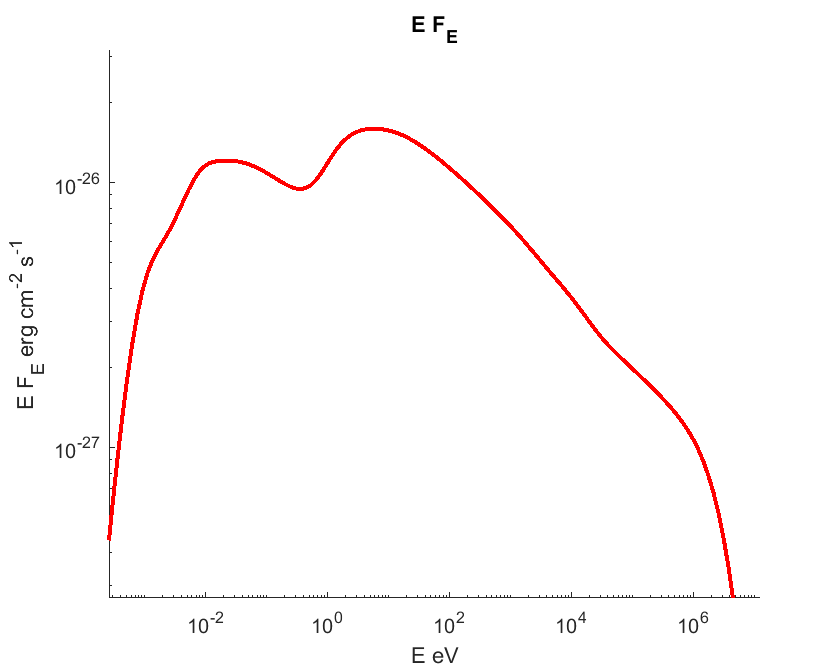
\includegraphics[width=12.5 cm]{./fig/compton.png} 
	\caption{Расчетная энергетическая плотность потока гамма излучения Кокона Лебедя и данные наблюдений}
	\label{pion}
\end{figure}
\section{Тормозное излучение}
В текущей версии кода реализовано вычисление тормозного излучения электронов в плазме только для случая теплового распределения. Для этого предназначен класс BremsstrahlungThermalEvaluator. В процессе расчета предполагается, что плазма электрон-протонная, с одинаковыми температурами электронов и протонов, в вычислении используются Гаунт-факторы, приведенные в \cite{Rybicki}. Пример вычисления тормохного излучения приведен в функции evaluateBremsstrahlung в файле examples.cpp.

